\chapter{Introducción}

\href{https://git-scm.com/}{Git} es un sistema de control de versiones distribuido creado en 2005 por Linus Torvalds, el mismo creador del kernel Linux. En tres días el sistema de control de versiones ya estaba versionando su propio código, y en dos semanas ya tenía gestión de ramas.

El proyecto se inició debido a que el sistema que utilizaban para la gestión del kernel Linux (Bitkeeper, en ese momento software privativo) decidió dejar de dar licencias gratuitas a los desarrolladores de Software Libre.

Linus hizo un análisis de los sistemas de control que existían en ese momento, y al ver que ninguno se adaptaba a las necesidades de un sistema tan complejo como el proyecto Linux, decidió crear uno propio.

Para el 16 de junio de 2005, Git manejaba el código fuente completo del kernel Linux, siendo el sistema utilizado a partir de ese momento. No sólo los cambios a partir de ese momento, si no que habían portado todo el histórico de cambios de los últimos 14 años.

\chapter{Características}

Git es un proyecto que ha crecido y ha añadido nuevas características, pero desde el inicio las más importantes fueron:

\begin{itemize}
    \item Sistema \textbf{distribuido}, por lo que cada desarrollador tiene una copia completa de todo el histórico y los cambios sin necesidad de necesitar acceso a internet.

    \item Compatible con los sistemas y protocolos actuales, como HTTPS, FTP y SSH.

    \item Debe permitir \textbf{desarrollos no lineales}, donde se permita crear ramas y unirlas de manera rápida y eficiente.

    \item \textbf{Eficiente} con proyectos grandes y gran cantidad de ficheros y desarrolladores. Al final, el propósito inicial era usarlo para el kernel Linux donde había miles de ficheros y desarrolladores.

    \item Los identificadores de los commits están basados en criptografía (SHA1). De esta manera no puedan existir dos commits con el mismo ID, y un ID representa única y exclusivamente un commit.
\end{itemize}


\chapter{Instalación}

Git está presente en todos los sistemas operativos actuales. Dependiendo del sistema operativo que utilicemos, podremos instalarlo de distintas maneras. En la  \href{https://git-scm.com/download/}{web oficial} están las últimas versiones.

Podemos hacer uso de Git a través de sistemas de consola o de aplicaciones gráficas. Hoy en día los entornos de desarrollo más conocidos también lo tienen integrado, por lo que es posible hacer uso de Git desde ellos.

\begin{itemize}
    \item Windows:
    \begin{itemize}
        \item \href{https://gitforwindows.org/}{Git Bash}
    \end{itemize}
    \item MacOS:
    \begin{itemize}
        \item MacOS tiene integrado Git dentro de las herramientas de desarrollador de Xcode. Para instalar únicamente Git desde un terminal debemos ejecutar:  \commandbox{xcode-select --install}
        \item Como mejor opción se recomienda usar \href{https://brew.sh/}{Brew.sh} e instalarlo a través de él.
    \end{itemize}
    \item GNU/Linux:
    \begin{itemize}
        \item Hoy en día todas las distribuciones tienen en sus repositorios Git, por lo que lo recomendable es hacer uso del sistema de instalación propio (apt, yast, ...). También es probable que ya esté instalado.
    \end{itemize}
\end{itemize}


\chapter{Primeros pasos}

Una vez instalado, debemos realizar una pequeña configuración que después se utilizará cada vez que realicemos un commit: crear una identidad.

\begin{mycode}{Añadiendo nuestro nombre y e-mail}{console}{}
ruben@vega:~$ git config --global user.name "Ruben Gomez"
ruben@vega:~$ git config --global user.email ruben@example.com
\end{mycode}

Esta configuración se guarda dentro de un fichero de configuración en la carpeta raíz de nuestro usuario. El fichero es \configfile{.gitconfig}. En este fichero podremos añadir configuraciones que se aplicarán a los comandos que realicemos.

A nivel de configuración podemos llegar a tener configuraciones específicas globales, del sistema, del repositorio y del área de trabajo, pero no entraremos en ello.

\chapter{Estado de los ficheros}
Dentro del repositorio, los ficheros que vayamos creando y/o modificando pueden estar en distintos estados. Esto es lo que se denomina “ciclo de vida” o \textit{lifecycle} de un fichero.Los ficheros pueden estar en los siguientes estados:

\begin{itemize}
    \item \textbf{Sin seguimiento}: Es un fichero nuevo que no está en seguimiento por el sistema de control de versiones. Aunque se realicen cambios en él, no podremos volver a versiones previas. En caso de usar un repositorio remoto, este fichero no estará en él.

    \item \textbf{Con seguimiento}: Estos ficheros pueden estar en los siguientes estados:
    \begin{itemize}
        \item \textbf{Sin modificar}: El fichero no ha sufrido modificaciones desde el último commit.
        \item \textbf{Modificado}: El fichero tiene modificaciones.
        \item \textbf{Preparado}: En inglés “staged”. Es un área donde se encuentran los ficheros que van a ir en el siguiente commit.
    \end{itemize}
\end{itemize}

En esta imagen se puede ver cómo los ficheros pueden cambiar de estado, y desde qué estado pasar a otro:

\begin{center}
    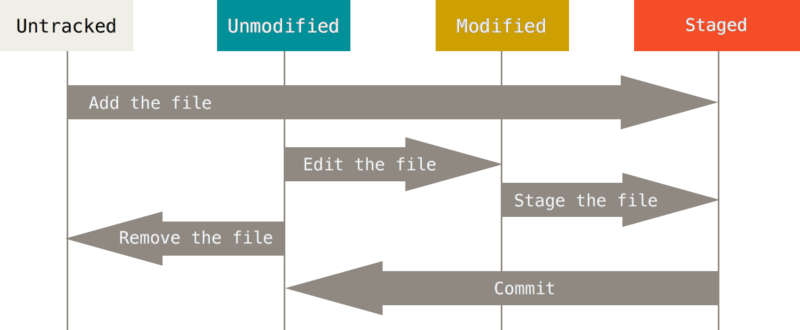
\includegraphics[width=0.9\linewidth]{lifecycle.png}
    \captionof{figure}{Estado de los ficheros. \href{https://git-scm.com/book/en/v2/Git-Basics-Recording-Changes-to-the-Repository}{Fuente}.}
\end{center}

Para entender esto mejor lo veremos a medida que vayamos haciendo uso de los comandos y creando/modificando ficheros.

\chapter{Comandos básicos}

Vamos a crear un repositorio para empezar a entender qué es lo que sucede con los ficheros que vamos creando en él, y tratar de entender los comandos más básicos.

\section{Crear repositorio local}

Vamos a crear un repositorio local dentro de un directorio nuevo, donde crearemos un proyecto que queremos versionar. Todo ello lo vamos a hacer dentro de un directorio nuevo llamado \configdir{pruebas}.

\begin{mycode}{Crear un repositorio git}{console}{}
ruben@vega:~$ mkdir pruebas
ruben@vega:~$ cd pruebas
ruben@vega:~/pruebas$ git init
Inicializado repositorio Git vacío en /home/ruben/pruebas/.git/

ruben@vega:~/pruebas$ ls -a
.  ..  .git/
\end{mycode}

Tal como se puede ver, ejecutando \commandbox{git init} dentro del directorio, nos inicializa el repositorio. Podemos ver que nos ha creado un directorio \configdir{.git}, que es un directorio oculto donde dentro se guarda la configuración y los commits que iremos realizando.

\errorbox{\textbf{No hagas cambios (ni borres nada) dentro del directorio .git}}


\section{Crear primer commit}

Con nuestro editor de textos favoritos, vamos a crear un fichero \configfile{README.md}. Normalmente este fichero es creado para indicar (en formato \href{https://es.wikipedia.org/wiki/Markdown}{Markdown}) información acerca del contenido del proyecto, qué es, para qué sirve, cómo compilarlo/usarlo...

Una vez creado el fichero vamos a entender qué es lo que está sucediendo dentro del repositorio:

\begin{mycode}{Comprobar estado del repositorio}{console}{}
ruben@vega:~/pruebas$ git status
En la rama main
No hay commits todavía

Archivos sin seguimiento:
(usa "git add <archivo>..." para incluirlo a lo que será confirmado)
README.md

no hay nada agregado al commit pero hay archivos sin seguimiento
presentes (usa "git add" para hacerles seguimiento)
\end{mycode}


Vemos que el estado del único fichero que hemos creado es “sin seguimiento” (tal como hemos explicado en el punto anterior). Es momento de pasar nuestro fichero a estado “preparado”, para ello:

\begin{mycode}{Preparamos el fichero para hacer commit}{console}{}
ruben@vega:~/pruebas$ git add README.md
ruben@vega:~/pruebas$ git status
En la rama main
No hay commits todavía

Cambios a ser confirmados:
(usa "git rm --cached <archivo>..." para sacar del área de stage)
nuevos archivos: README.md
\end{mycode}

El fichero \configfile{README.md} está en el área “stage”, por lo que ahora es el momento en el que podemos hacer nuestro primer commit con las modificaciones realizadas:


\begin{mycode}{Hacemos el commit}{console}{}
ruben@vega:~/pruebas$ git commit -m "Primer commit"
[main (commit-raíz) 45900ae] Primer commit
1 file changed, 3 insertions(+)
create mode 100644 README.md

guruben@vega:~/pruebas$ git status
En la rama main
nada para hacer commit, el árbol de trabajo está limpio
\end{mycode}

Con \commandbox{git commit -m “Primer commit”} lo que estamos es “encapsulando” todas las modificaciones de todos los ficheros que están en el área “stage” (en este caso un único fichero), y vamos a generar un commit al que le hemos puesto el mensaje “Primer commit”.


\section{Ver histórico de cambios}
Si realizamos varios cambios al fichero, o si añadimos un fichero nuevo y realizamos una serie de commits, nos puede interesar saber cómo está yendo el histórico de commits.

Para ello podemos hacer uso del comando \commandbox{git log}, que nos mostrará en orden por fecha descendente, todos los commits que ha tenido nuestro repositorio:

\begin{mycode}{Ver histórico de commits}{console}{}
ruben@vega:~/pruebas$ git log

commit ac00ce47dcdcda01bf33d162890bd98cc4f36ead (HEAD -> main)
Author: Rubén Gómez <ruben@example.com>
Date:   Sun Sep 17 10:52:26 2023 +0200

Añadir hola.java

commit a3f9554e0917dfdd2ce6ccccb5957d44d63c7f6f
Author: Rubén Gómez <ruben@examplel.com>
Date:   Sun Sep 17 10:52:03 2023 +0200

Añadir datos a README

commit 45900aef0300bf88c3a2939b8cf2f6b05de572dc
Author: Rubén Gómez <ruben@example.com>
Date:   Sun Sep 17 10:46:12 2023 +0200

Primer commit
\end{mycode}

De manera gráfica, el histórico de los \textit{commits} podríamos representarlo de la siguiente manera:

\begin{center}
    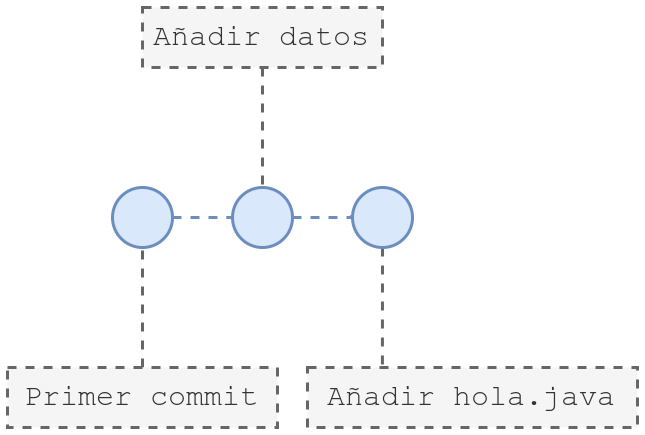
\includegraphics[width=0.6\linewidth]{log.png}
    \captionof{figure}{Estado tras varios commits}
\end{center}